\documentclass{beamer}
\usepackage{../common_slides}
\setbeamercovered{invisible}
\title{Text Classification\\ + \\ Machine Learning Review 3 }
\date{}
\author{CS 287}
\begin{document}

\begin{frame}
  \titlepage
\end{frame}

\begin{frame}{Review:  Logistic Regression (Murphy, p 268)}
  \textcolor{red}{Cons}
  \begin{itemize}
  \item Harder to fit versus naive Bayes.
  \item Must fit all classes together.
  \item Not a good fit for semi-supervised/missing data cases

  \end{itemize}
  \textcolor{blue}{Pros}
  \begin{itemize}
  \item Better calibrated probability estimates
  \item Natural handling of feature input 
 
    \begin{itemize}
    \item Features likely not multinomials
    \end{itemize}

  \item (For us) extend naturally to neural networks 
  \end{itemize}
\end{frame}



\begin{frame}{Review: Gradients for Softmax Regression}

  For multiclass logistic regression:
  
  \[ \frac{\partial L(\boldy, \hat{\boldy})}{\partial z_i} = \sum_{j} \frac{\partial \hat{y}_j }{\partial z_i}  \frac{\indicator(j = c)} {\hat{y}_j} =     \begin{cases}
      -(1 - \hat{y}_i) & i = c\\
      \hat{y}_i & ow. \\
    \end{cases} \] 

  Therefore for parameters $\theta$, 

  \[\frac{\partial L}{\partial b_{i}} = 
    \frac{\partial L}{\partial z_{i}} \ \ \ \ \frac{\partial L}{\partial W_{f, i}} = 
     x_f \frac{\partial L}{\partial z_{i}}\]

   \pause
   Intuition:
   \begin{itemize}
   \item Nothing happens on correct classification.
   \item Weight of true features increases based on prob not given.
   \item Weight of false features decreases based on prob given.
   \end{itemize}
\end{frame}


\begin{frame}{Gradient-Based Optimization: SGD}
  \begin{figure}
    \begin{algorithmic}
      \Procedure{SGD}{}
      \While{training criterion is not met}
      \State{Sample a training example $\boldx_i, \boldy_i$}
      \State{Compute the loss $L(\hat{\boldy}_i, \boldy_i;\theta)$}
      \State{Compute gradients $\hat{\boldg}$ of $L(\hat{\boldy}_i, \boldy_i;\theta)$ with respect to $\theta$}
      \State{$\theta \gets \theta - \eta \hat{\boldg}$}
      \EndWhile{}
      \State{\Return{$\theta$}}
      \EndProcedure{}
    \end{algorithmic}
  \end{figure}
\end{frame}


\begin{frame}{Quiz: Softmax Regression}
  Given bag-of-word features \[\mcF = \{\mathrm{\texttt{The, movie, was, terrible, rocked, A}} \}\] and two training data points:
    
  \begin{center}
    Class 1: \texttt{The movie was terrible}
  
    Class 2: \texttt{The movie rocked}
  \end{center}
  \\

  \air 

  Assume that we start with parameters $\boldW = 0$ and $\boldb = 0$,
  and we train with learning rate $\eta = 1$ and $\lambda = 0$. What is
  the loss and the parameters after one pass through the data in order?
\end{frame}

\begin{frame}{Answer: Softmax Regression (1) }
  First iteration,
  \[\hat{\boldy}_1 = \begin{bmatrix} 0.5 & 0.5 \end{bmatrix}\]

  \[ L(\boldy_1, \hat{\boldy}_1) = - \log 0.5 \]

  \[ \boldW =
  \begin{bmatrix}
    0.5 & 0.5 & 0.5 & 0.5 & 0 & 0 \\
    -0.5 & -0.5 & -0.5 & -0.5 & 0 & 0 \\
  \end{bmatrix}
  \]

  
  \[ \boldb =
  \begin{bmatrix}
    0.5 & -0.5 \\
  \end{bmatrix} \]
\end{frame}


\begin{frame}{Answer: Softmax Regression (2) }
  Second iteration,

  \[\hat{\boldy}_1 = \softmax([1.5\ -1.5] ) \approx \begin{bmatrix} 0.95 &  0.05  \end{bmatrix}\]

  \[ L(\boldy_2, \hat{\boldy}_2) = - \log 0.05 \]

  \[ \boldW \approx
  \begin{bmatrix}
    -0.45 & -0.45 & 0.5 & 0.5 & -0.95 & 0 \\
     0.45 & 0.45 & -0.5 & -0.5 & 0.95 & 0 \\
  \end{bmatrix}
  \]

  \[ \boldb =
  \begin{bmatrix}
    -0.45 & 0.45 \\
  \end{bmatrix} \]
\end{frame}


\begin{frame}{Today's Class}
  So far
  \begin{itemize}
  \item Naive Bayes (Multinomial)
  \item Multiclass Logistic Regression (SGD)
  \end{itemize}

  Today

  \begin{itemize}
  \item Multiclass Hinge-loss
  \item More about optimization
  \end{itemize}
\end{frame}


\section{Multiclass Hinge-Loss}

\begin{frame}{Other Loss Functions}
  
  What if we just try to directly find $\boldW$ and $\boldb$? 
     \[\hat{\boldy} = \boldx \boldW + \boldb\]   
     
     \begin{itemize}
     \item No longer a probabilistic interpretation.
     \item Just try to find parameters that fit training data.
     \end{itemize}

\end{frame}

\begin{frame}{0/1 Loss}
  Just count the number of training examples we classify correctly,  
  \[{\mathcal{L}(\theta)} = \sum_{i=1}^n L_{0/1}(\boldy, \hat{\boldy}) = \indicator(\argmax_{c'} \hat{y}_{c'} \neq c)   \]

  \pause
\[ \frac{\partial L(\boldy, \hat{\boldy})}{\partial \hat{y}_j} = \begin{cases}0 & j = c\\ 0 & o.w. \end{cases}  \]

      \begin{figure}
        \centering
      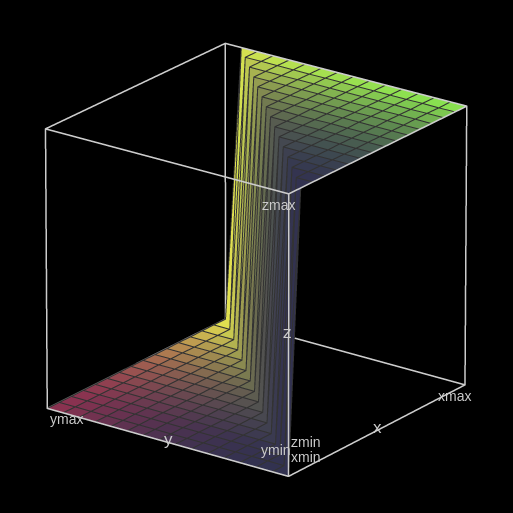
\includegraphics[width=3cm]{argmax}
      \end{figure}
      \[L_{0/1}([x\ y]) = \indicator(x > y) \]      

\end{frame}


% \begin{frame}{0/1 Loss}
  

%   \[ L_{0/1}(\boldy, \hat{\boldy}) =  \indicator(\argmax_{c'} \hat{y}_{c'} \neq c)   \]


% \[ \frac{\partial L(\boldy, \hat{\boldy})}{\partial \hat{y}_j} = \begin{cases}0 & j = c\\ 0 & o.w. \end{cases}  \]

%       \begin{figure}
%         \centering
%       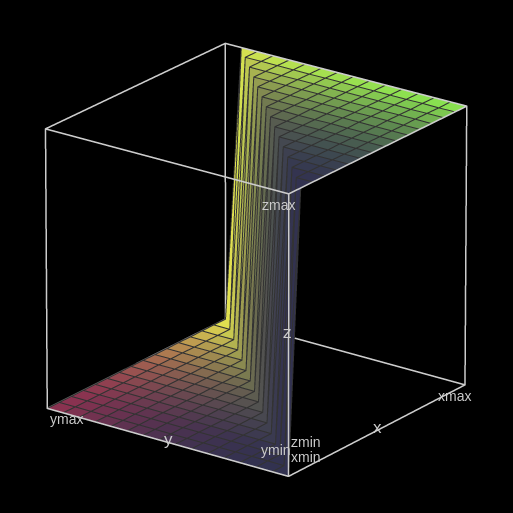
\includegraphics[width=3cm]{argmax}
%       \end{figure}
%       \[L_{0/1}([x\ y]) = \indicator(x > y) \]      

% \end{frame}


\begin{frame}{Hinge Loss}

  \[{\mathcal{L}(\theta)} = \sum_{i=1}^n L_{hinge}(\boldy,\hat{\boldy}) \] 


  \[ L_{hinge}(\boldy, \hat{\boldy}) =  \max\{0, 1 - (\hat{y}_{c} - \hat{y}_{c'}) \}  \]

  Where 
  \begin{itemize}
  \item   Let $c$ be defined as true class $y_{i, c} = 1$  
    \[c' = \argmax_{i \in \mcC \setminus\{c\}} \hat{y}_i \] 
  \end{itemize}

  \pause

  Minimizing hinge loss is an upper-bound for 0/1. 

  \[ L_{hinge}(\boldy, \hat{\boldy}) \geq L_{0/1}(\boldy, \hat{\boldy})\] 
\end{frame}
\begin{frame}{Hinge Loss}
  \begin{columns}[t]
    \begin{column}[t]{0.5\textwidth}


      \begin{figure}
        \centering
        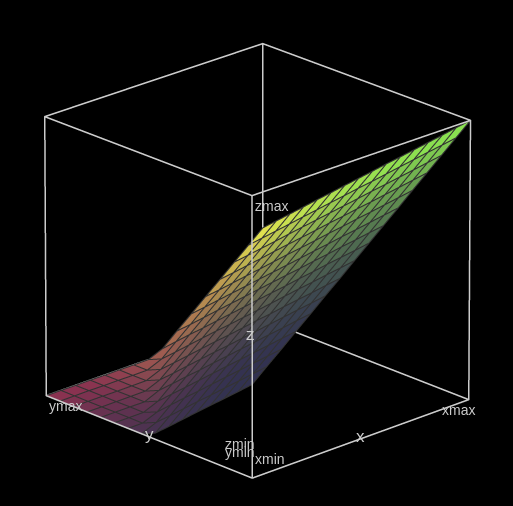
\includegraphics[width=5cm]{hinge}

      \end{figure}
      \[\mathrm{hinge}(\hat{\boldy}) = \indicator(\max\{0, 1 - (y - x)\}) \]
    \end{column}

    \begin{column}[t]{0.5\textwidth}


      \begin{figure}
        \centering
      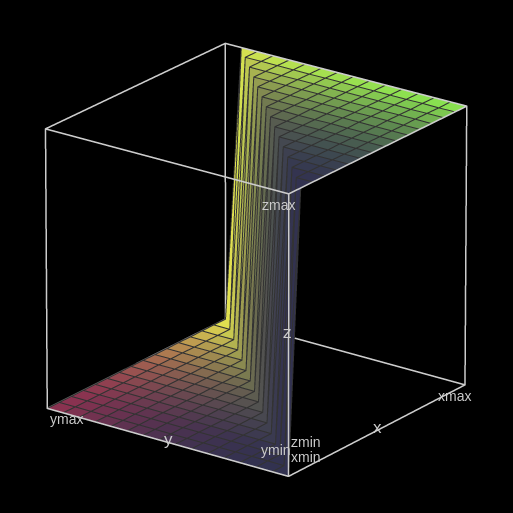
\includegraphics[width=5cm]{argmax}
      \end{figure}
      \[\argmax([x\ y]) = \indicator(x > y) \]      
    \end{column}
  \end{columns}
\end{frame}  


\begin{frame}{Important Case: Hinge-loss for Binary }
  \[L_{hinge}([0\ 1], [x\ y]) = \max\{0, 1 - (y -x) \} = \relu(1 -(y-x)) \] 


  Neural network name (Rectified linear unit):

  \[\relu(t) = \max\{0, t\}  \]

  \begin{figure}
    \centering
    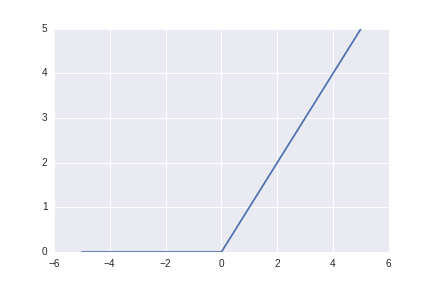
\includegraphics[width=5cm]{Relu}
  \end{figure}

\end{frame}



% \begin{frame}{Hinge Loss}
%   For a given example $\boldy_i$,

%   \begin{itemize}
%   \item   Where $c$ is gold class $y_{i, c} = 1$  
%   \item    $\bar{c}$ is the highest scoring non-gold class 
%     \[\bar{c} = \argmax_{c \in \mcC \setminus\{c\}} \hat{y}_c \] 
%   \end{itemize}


%     \[ \mathcal{L}_{margin}(\theta) = \sum_{i=1}^n \max\{0, 1 - \hat{y}_{i, c} + \hat{y}_{i, \bar{c}}\}  + ||\theta||^2_2 \]
% \end{frame}


\begin{frame}{Hinge-Loss Properties}
  Complete objective:
  \begin{eqnarray*}
     \mathcal{L}_{hinge}(\theta) &=& \sum_{i=1}^n \max\{0, 1 - (\hat{y}_{c} - \hat{y}_{c'})\} \\
    &=& \sum_{i=1}^n \max\{0,  1 - (\hat{y}_{c} - \max_{c' \in \mcC \setminus\{c\}} \hat{y}_{c'}) \}     
  \end{eqnarray*}


  \begin{itemize}
  \item Apply convexity rules: Linear $\hat{\boldy}$ is convex, 
    max of convex functions is convex, linear + convex is convex, sum of convex functions is convex (Boyd and  Vandenberghe, 2004 p. 72-74)
  \item However, non-differentiable because of max.
  \end{itemize}
\end{frame}

\begin{frame}{Piecewise Linear Objective}
    \[\mathcal{L}(\theta) = \sum_{i=1}^n \max\{0, 1 - (\hat{y}_{c} - \hat{y}_{c'})\}   \]

  \begin{center}
    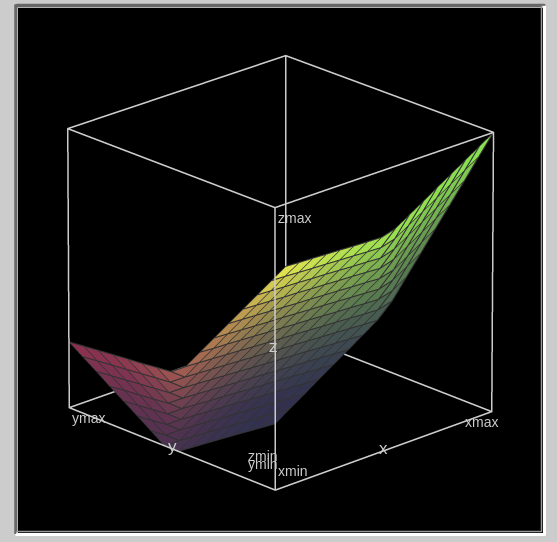
\includegraphics[width=5cm]{hingenol2}
    \[10*\max\{0,1 - (y-x)\}+5*\max\{0,1-(x-y)\}\]
  \end{center}
\end{frame}

\begin{frame}{Objective with Regularization}
    \[\mathcal{L}(\theta) = \sum_{i=1}^n \max\{0, 1 - (\hat{y}_{c} - \hat{y}_{c'})\}  + \lambda ||\theta||^2 \]
  \begin{center}

    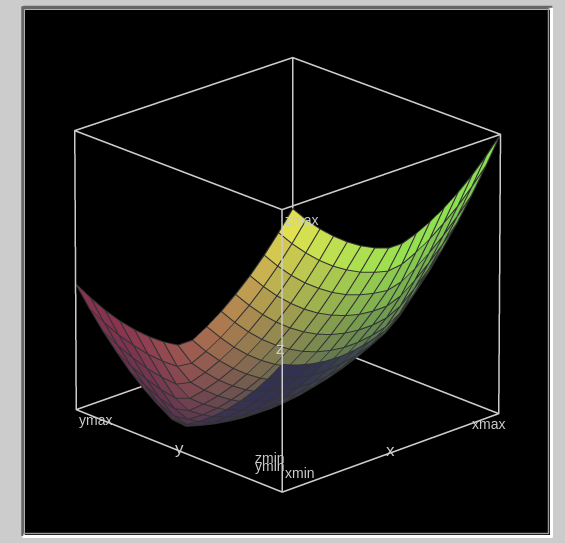
\includegraphics[width=5cm]{hingel2}

    \[10*\max\{0,1 - (y-x)\}+5*\max\{0,1-(x-y)\}+5*||\theta||^2\]
  \end{center}
\end{frame}

\section{Gradients}

\begin{frame}{(Sub)Gradient Rule}

  \begin{itemize}
  \item Technically $\relu$ is non-differentiable.
  \item Only an issue at $0$, generally for ``ties''.
  \item We informally use subgradients, 
    
    \[\frac{d \relu(x)}{d x} =
      \begin{cases}
         1 & x > 0 \\
         0 & x < 0 \\
         1 \mathrm{\ or\ } 0 & o.w \\
      \end{cases}
    \]

    Generally,
    \[\frac{d \max_{v'}(f(x, v'))}{d x} = f'(x, \hat{v}) \ \mathrm{for\ any} \ \hat{v} \in \argmax_{v'} f(x, v')
    \]
    
  \end{itemize}
\end{frame}

\begin{frame}{Symbolic Gradients}

  \begin{itemize}
  \item   Let $c$ be defined as true class
  \item   Let $c'$ be defined as the highest scoring non-true class 
    \[c' = \argmax_{i \in \mcC \setminus\{c\}} \hat{y}_i \] 
  \item Partials of $L(y, \hat{y})$

  \[ \frac{\partial L(y,k \hat{y})}{\partial \hat{y}_j} =
      \begin{cases}
         0 & \hat{y}_c - \hat{y}_{c'} > 1  \\
         1 & j = c' \\
         -1 & j = c \\
         0 & o.w. \\ 
      \end{cases}
  \]
  \end{itemize}
  Intuition: If wrong or close to wrong, improve correct and lower closest incorrect.
\end{frame}


\begin{frame}{Notes: Hinge Loss: Regularization}
  \begin{itemize}
  \item   Many different names,
  \begin{itemize}
  \item Margin Classifier
  \item Multiclass Hinge
  \item Linear SVM
  \end{itemize}

  \item Important to use regularization.  
  \[ \mathcal{L}(\theta) = - \sum_{i=1}^n L(\hat{\boldy}, \boldy) + ||\theta||^2_2\] 

  \item Can be much more efficient to train than LR. (No partition).

  \end{itemize}
\end{frame}

\begin{frame}{Results: Longer Reviews}
  \begin{figure}
    \centering
    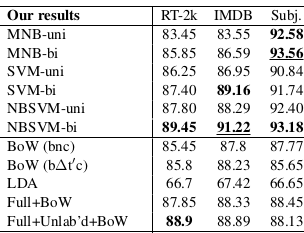
\includegraphics{svm}
    \caption{IMDB (longer movie review), Subj (longer subjectivity)}
  \end{figure}

  \begin{itemize}
  \item NBSVM is hinge-loss interpolated with Naive Bayes.
  \end{itemize}
\end{frame}


\section{Black-Box Optimization}


% \begin{frame}{Black-Box Optimization Methods}
%   Brief tour of optimization methods used in ML and NLP.
%   % \begin{center}
%   %   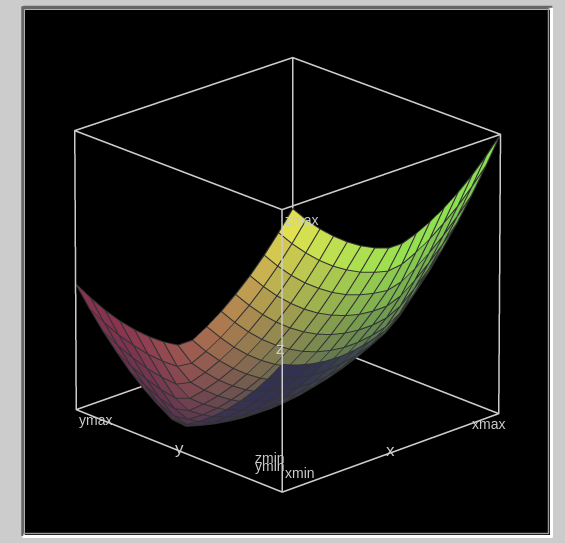
\includegraphics[width=5cm]{hingel2}
%   % \end{center}
% \end{frame}

\begin{frame}{Optimization Methods}
  \air
  \textbf{Goal:} Minimize function $\mathcal{L}: \reals^{|\theta|} \mapsto \reals $
  \air
  



  First-order Methods
  \[\mathcal{L}(\theta + \bolddelta) \approx \mathcal{L}(\theta) + L'(\theta)^\top \dot \bolddelta\]

  \begin{itemize}
  \item Require computing $L(\theta)$ and gradient $L'(\theta)$.
  \end{itemize}

  Second-order Methods
  \[\mathcal{L}(\theta + \bolddelta) \approx \mathcal{L}(\theta) + L'(\theta)^\top \bolddelta + 1/2 \bolddelta^\top \boldH \bolddelta^\top \]

  \begin{itemize}
  \item  Require computing $L(\theta)$ and gradient $L'(\theta)$ and Hessian $\boldH$.
  \end{itemize}

  Stochastic Methods
  \begin{itemize}
  \item  Require computing $\mathbb{E}(L(\theta))$ and expected gradient.
  \end{itemize}
\end{frame}


\begin{frame}{Gradient Descent}
  \begin{figure}
    \begin{algorithmic}
      \While{training criterion is not met}
      \State{$k \gets 0$}
      \State{$\hat{\boldg} \gets 0$}
      \For{$i = 1 \mathrm{\ to\ } n$}
      \State{Compute the loss $L(\hat{\boldy}_i, \boldy_i;\theta)$}
      \State{Compute gradients $\boldg'$ of $L(\hat{\boldy}_i, \boldy_i;\theta)$ with respect to $\theta$}
      \State{$\hat{\boldg} \gets \hat{\boldg} +  \frac{1}{n} \boldg'$}
      \EndFor{}
      \State{$\theta_{k+1} \gets \theta_{k} - \eta_k \hat{\boldg}$}
      \State{$k \gets k + 1$}
      \EndWhile{}
      \State{\Return{$\theta$}}
    \end{algorithmic}
  \end{figure}  
\end{frame}

\begin{frame}{Choosing the Learning Rate}
  \begin{center}
    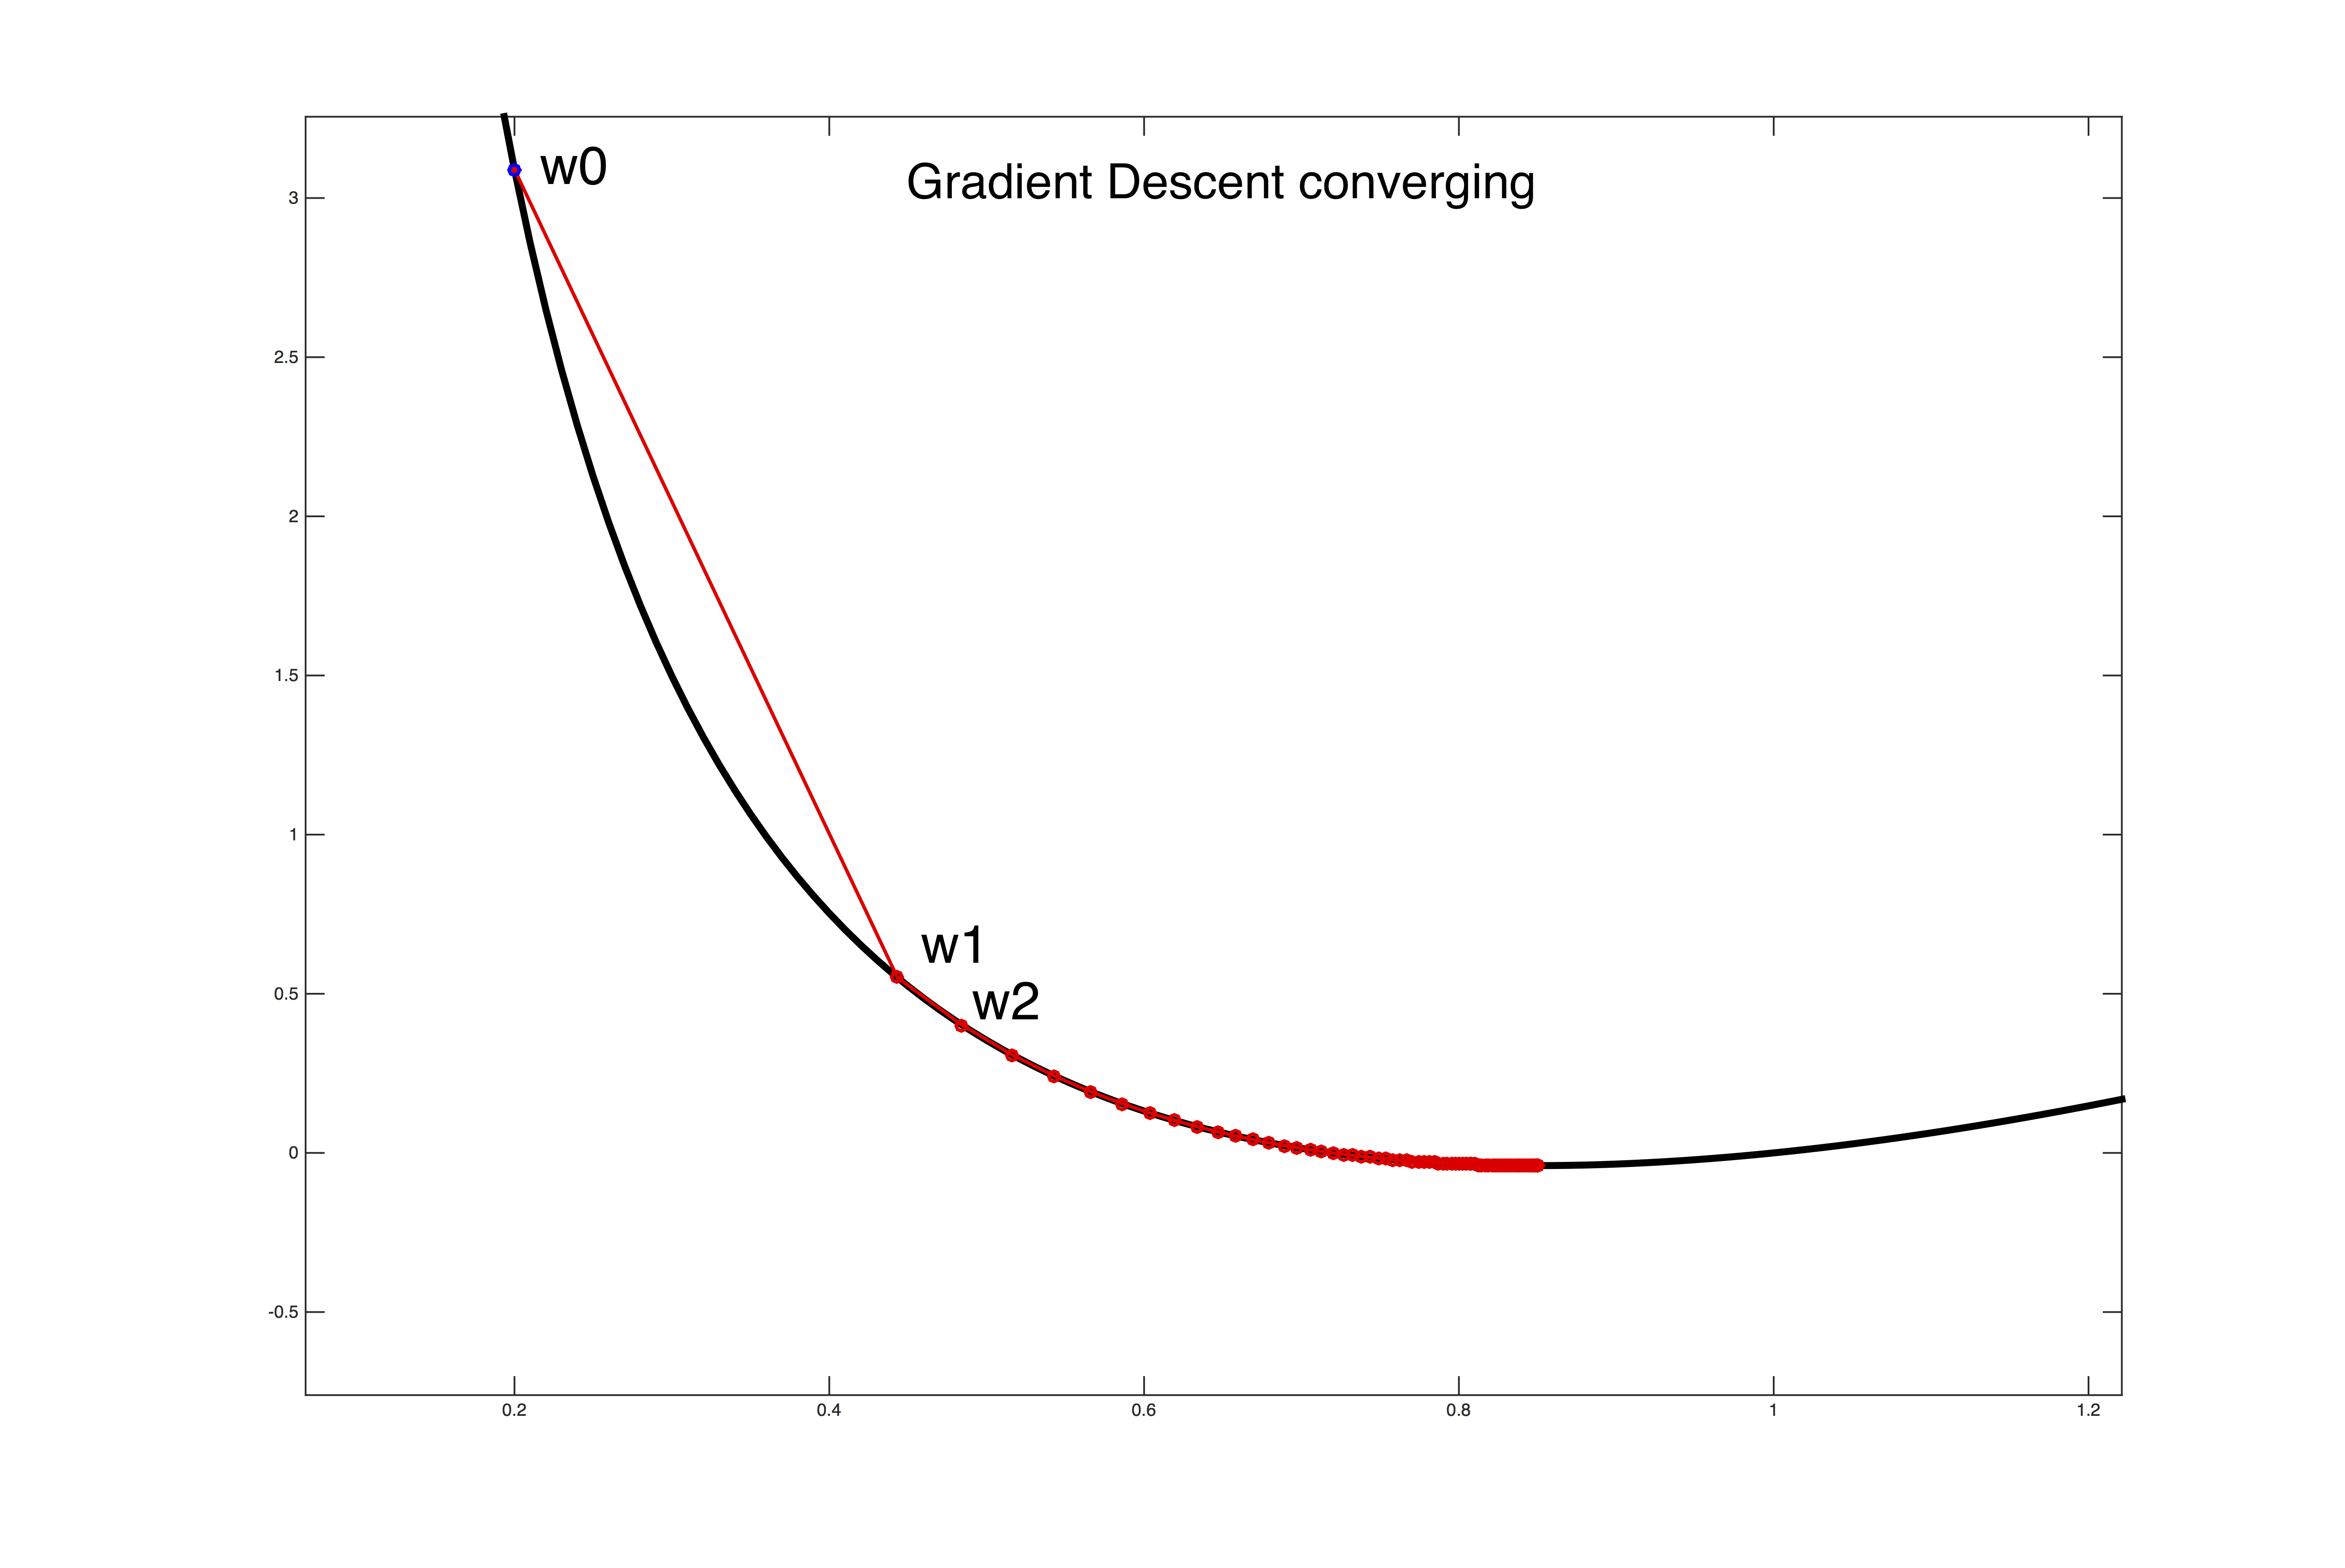
\includegraphics[width=4cm]{converge}
    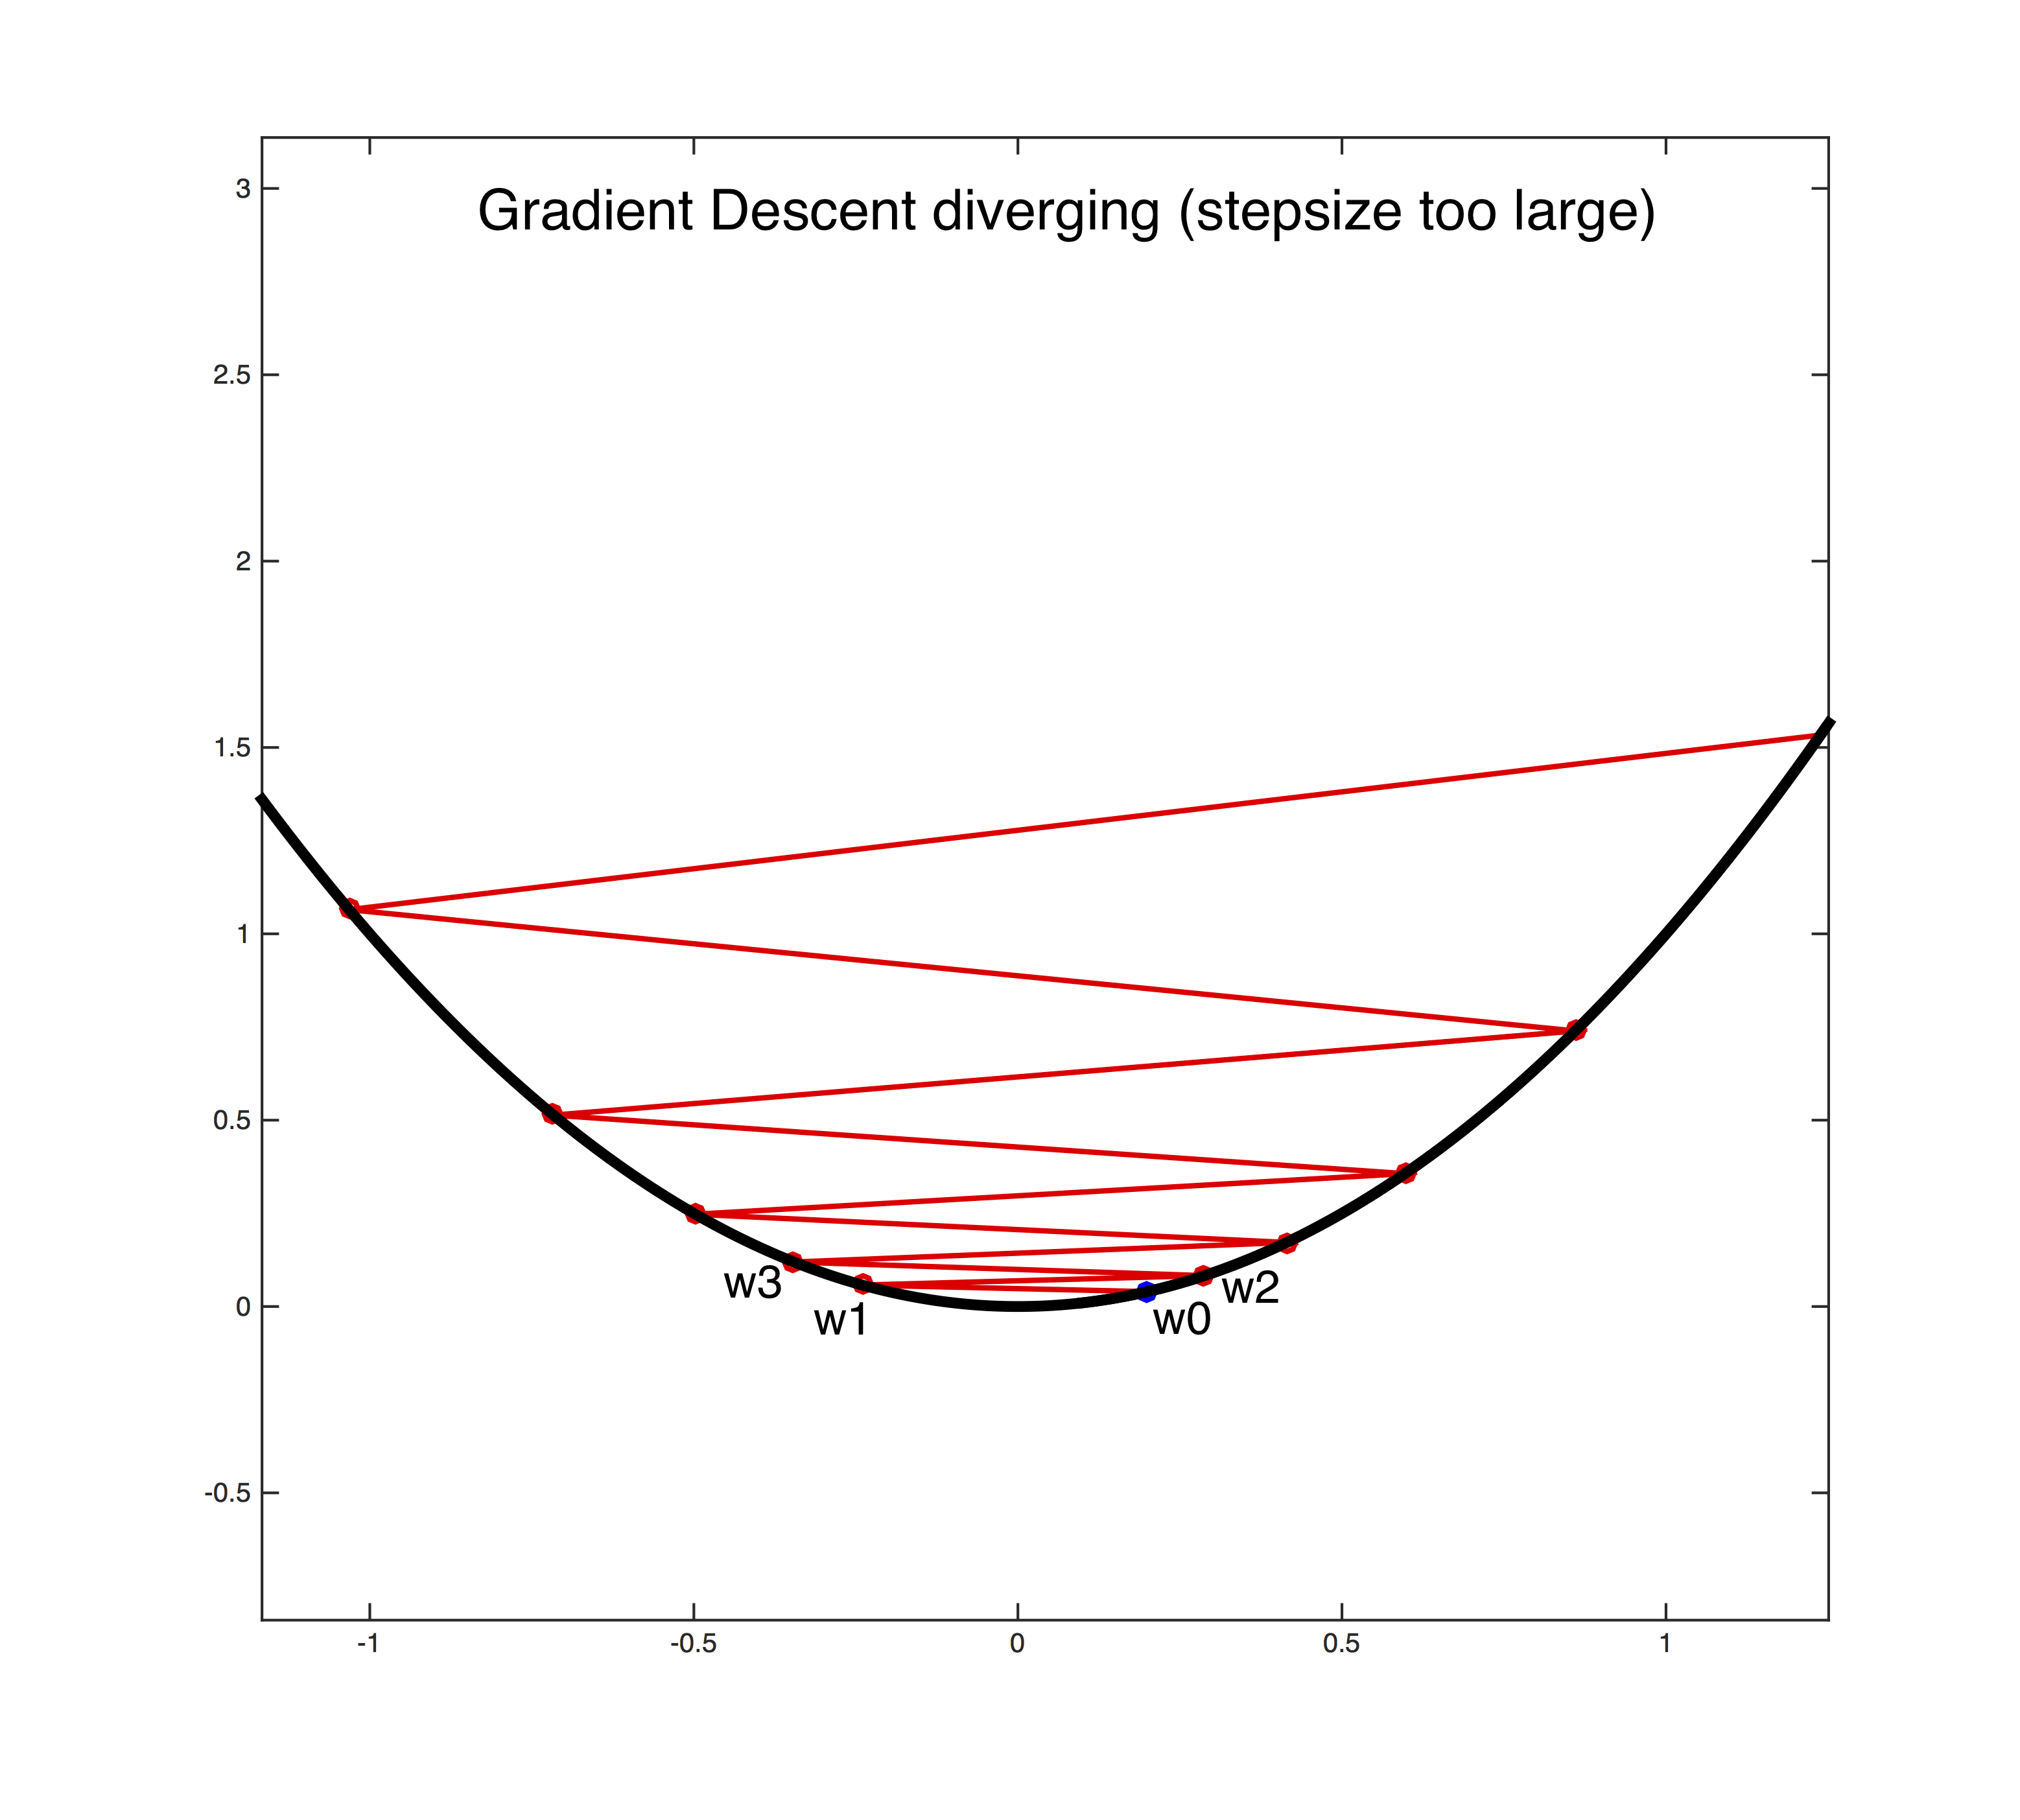
\includegraphics[width=4cm]{diverge}
  \end{center}
  

  \begin{center}
    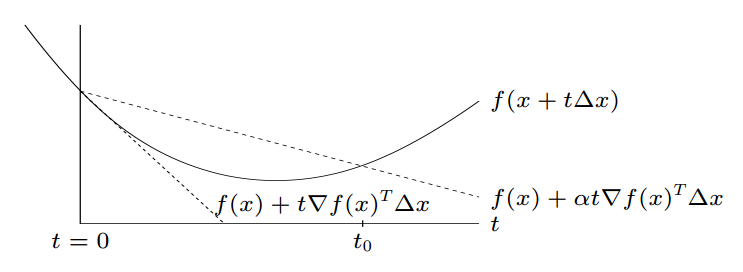
\includegraphics[width=7cm]{grad}
  \end{center}
\end{frame}


\begin{frame}{Gradient Descent with Momentum}
  Standard Gradient Descent (figure from Boyd):
  \[\theta_{k+1} \gets \theta_{k} - \eta_k \hat{\boldg}\]

  \begin{center}
    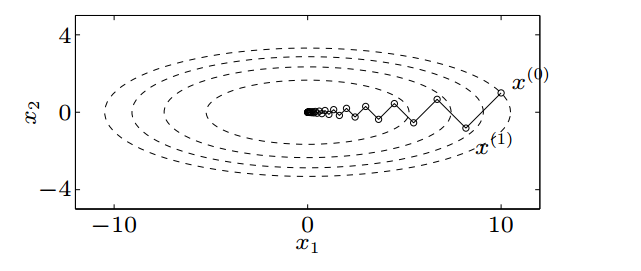
\includegraphics[width=9cm]{heavyball}
  \end{center}

  Momentum terms:
  \[\theta_{k+1} \gets \theta_{k} - \eta_k \hat{\boldg} + \mu_k(\theta_{k} - \theta_{k-1}) \]

  \begin{itemize}
  \item Also known as: Heavy-ball method
  \end{itemize}
\end{frame}

\begin{frame}{Second-Order}

  Requires  compute Hessian $\hat{\boldH}$ 

   Second-order update becomes:
  \[\theta_{k+1} \gets \theta_{k} - \eta_k \hat{\boldH}^{-1} \hat{\boldg} \]


  \begin{center}
    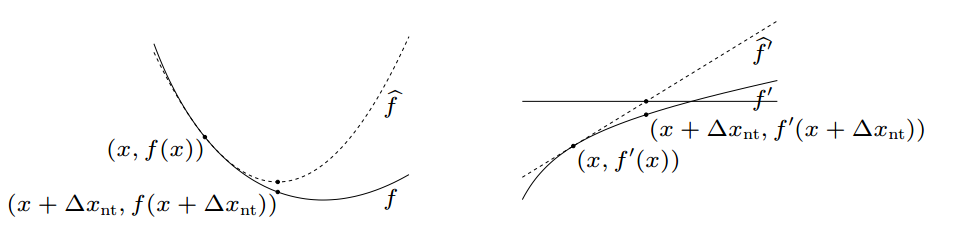
\includegraphics[width=8cm]{newton}
  \end{center}
  \begin{itemize}
  \item Used for strictly convex functions (although there are variants)
  \item Also known as: Newton's Method
  \end{itemize}

\end{frame}


% \begin{frame}{Second-Order Methods}
%   \begin{itemize}
%   \item In practice, second-order methods are often infeasible.
%   \item Simply storing the Hessian is $O(|\theta|^2)$.
%   \item However, first-order methods are quite slow.
%   \end{itemize}
% \end{frame}


\begin{frame}{Quasi-Newton Methods  }
  Construct an approximate Hessian from  first-order information
  \begin{itemize}
  \item BFGS 
    \begin{itemize}
    \item construct approx. Hessian directly
    \item $O(|\theta|^2)$ space
    \end{itemize}

  \item L-BFGS; 
    \begin{itemize}
    \item limited-memory BFGS, only save last $m$ gradients
    \item can often set $m <20$ or smaller
    \end{itemize}
  \end{itemize}
  
  Fast implementations available, specific details are beyond scope of course.

\end{frame}

\begin{frame}{Stochastic Methods}
  \begin{itemize}
  \item Minimize function $L(\theta)$
  \item Require computing $\mathbb{E}(L(\theta))$ and gradient
  \end{itemize}

  \begin{itemize}
  \item Typically, we by sampling a subset of the data.
    computing a gradient, and updating
  \item Other first-order optimizers (like momentum) can be used.
  \end{itemize}
\end{frame}

\begin{frame}{Gradient-Based Optimization: Minibatch SGD}
  \begin{figure}
    \begin{algorithmic}
      \While{training criterion is not met}
      \State{Sample a minibatch of $m$ examples $(\boldx_1, \boldy_1), \ldots, (\boldx_m, \boldy_m) $}
      \State{$\hat{\boldg} \gets 0$}
      \For{$i = 1 \mathrm{\ to\ } m$}
      \State{Compute the loss $L(\hat{\boldy}_i, \boldy_i;\theta)$}
      \State{Compute gradients $\boldg'$ of $L(\hat{\boldy}_i, \boldy_i;\theta)$ with respect to $\theta$}
      \State{$\hat{\boldg} \gets \hat{\boldg} +  \frac{1}{m} \boldg'$}
      \EndFor{}
      \State{$\theta \gets \theta - \eta_k \hat{\boldg}$}
      \EndWhile{}
      \State{\Return{$\theta$}}
    \end{algorithmic}
  \end{figure}
\end{frame}


\begin{frame}{Tricks On Using SGD (Bottou 2012)}
  \begin{itemize}


    \item Can be crucial to experiment with learning rate.
      \air 
    \item Often useful to use development set for stopping.
      \air
    \item Shuffle data first and run over it.
      \air
    \item Also describes ``averaged'' versions which work well in practice.

  \end{itemize}
\end{frame}

\begin{frame}{Optimization in NLP}
  \begin{itemize}
  \item For convex batch-methods:
    \begin{itemize}
    \item L-BFGS is easy to use and effective. 
    \item Nice for verifying results.
    \item Sometimes even $m$-times the parameters is a lot though.
    \end{itemize}
    
\air

  \item For both convex, and especially, non-convex problems:
    \begin{itemize}
    \item SGD and variants are dominant.
    \item Trade-off of speed vs. exact optimization.
    \item Also see notes on AdaGrad, another popular method.
    \end{itemize}
  \end{itemize}
\end{frame}

\end{document}  
